% Este archivo es parte de la memoria del proyecto fin de carrera
% de Manuel López Urbina. Protegida bajo la licencia GFDL.
% Para más información, la licencia completa viene incluida en el
% fichero fdl-1.3.tex

% Copyright (C) 2017 Manuel López Urbina

\newpage

\chapter{Introducción}
\label{chap:introducción}

\emph{Lo mejor que podemos hacer por otro\\ no es sólo compartir con él nuestras riquezas,\\ sino mostrarle las suyas\\ Benjamin Disraeli}\\


\section{Introducción y antecedentes}
\label{sec:introduccion_y_antecedentes}

La robótica es una rama de la ingeniería, la cual se ocupa del diseño, construcción, operación y uso de robots\footnote{Robot: Máquina automática programable capaz de 
realizar determinadas operaciones de manera autónoma y sustituir a los seres humanos en algunas tareas, en especial las pesadas, repetitivas o peligrosas; puede estar dotada de sensores, 
que le permiten adaptarse a nuevas situaciones.}, así como sistemas informáticos para su control, retroalimentación sensorial y procesamiento de información. Entre las diversas disciplinas aplicadas
a la robótica podemos encontrar: la mecánica, la electrónica, la informática, la inteligencia artificial, la ingeniería de control y la física, entre otras muchas, de lo cual podemos considerar 
la robótica como una ciencia multidisciplinar.\\

En la actualidad, los robots comerciales e industriales son ampliamente utilizados y cada día realizan tareas de forma más exacta o más barata que los humanos. También se les utiliza en trabajos demasiado sucios,
peligrosos o tediosos. Los robots son muy utilizados en plantas de fabricación, montaje y embalaje, en transporte, en exploraciones en la Tierra y en el espacio, cirugía, armamento, investigación en laboratorios y 
en la producción en masa de bienes industriales o de consumo. Otras aplicaciones incluyen la limpieza de residuos tóxicos, minería, búsqueda y rescate de personas y localización de minas terrestres. En definitiva, 
la robótica está presente en prácticamente cualquier ámbito que podamos imaginar.\\

Por otra parte, ninguno de los sistemas robóticos actuales podrían ser funcionales sin un software adecuado para su manejo y control, en ocasiones siendo éste tremendamente complejo y específico para garantizar
una correcta sincronización entre los diferentes elementos hardware y software implicados con la finalidad de garantizar una correcta armonía del conjunto.\\

Por estas razones cada vez son más las escuelas que hacen uso de la robótica para que los estudiantes se interesen en la tecnología, ya que pueden encontrar un entorno divertido donde aprender y que ofrece multitud de ventajas:\\

\begin{enumerate}
\item \textbf{Los niños lo encuentran divertido:} hay varios concursos orientados a distintos grupos de edad que pueden canalizar la competencia de una manera positiva. Por ejemplo, se le puede pedir a los niños que construyan un robot y luego hacer competiciones.\\
\item \textbf{Es una manera eficaz de enseñarles programación a los estudiantes:}
 la programación puede ser muy abstracta. Al tener que controlar un robot físico y ver lo que sale mal, los estudiantes aprenden lo que los robots pueden y no pueden hacer. 
También aprenden la necesidad de dar instrucciones precisas.\\
\item \textbf{ Desarrolla habilidades útiles:}
 capacidad de resolución de problemas, trabajo en equipo, capacidad de análisis, y un largo etcétera.
\end{enumerate}


Actualmente, además, existe una tendencia a la interconexión de aquellos elementos más cotidianos con internet, fenómeno conocido como Internet de las cosas o Internet of things en inglés. Con ello,
se permite el control de multitud de dispositivos, desde gestión de stocks, geolocalización, control remoto, y un largo etcétera de posibilidades. Según la empresa Cisco\footnote{Cisco Systems es 
una empresa global con sede en San José, California, Estados Unidos, principalmente dedicada a la fabricación, venta, mantenimiento y consultoría de equipos de telecomunicaciones.}, en 2020 habrá en
el mundo aproximadamente 50 mil millones de dispositivos con un sistema de conexión al internet de las cosas\footnote{ Estudio referenciado en el libro \textit{Internet of Things - From Research and Innovation to Market Deployment} 
\cite{book:internet_things}.} ¿Por qué no añadir también nuestros proyectos robóticos a la red?.\\

De todo lo anterior se extrae, por tanto, la necesidad de elaborar un sistema que, además de acercar la robótica a los estudiantes, permita compartir sus proyectos con otros usuarios en internet. Todos hemos
visto alguna vez vídeos en las redes sociales donde los usuarios nos muestran sus dispositivos en funcionamiento donde, en ocasiones, nos gustaría poder tomar control sobre ellos o visualizar su manejo en tiempo real.\\

Por tanto el sistema resultante debe cubrir dos necesidades principales, la primera, dotar al usuario de las herramientas necesarias para permitir la configuración de una interfaz de control para 
dispositivos sin necesidad de amplios conocimientos de programación, y la segunda, cubrir la necesidad paralela en la que los usuarios, orgullosos de sus creaciones, dispongan de una manera de 
compartir sus robots con el resto del mundo de una manera más dinámica. Es decir, en la que otros usuarios, a modo de espectadores, puedan visualizar el control de los dispositivos por parte de 
su creador, como si de una sesión de vídeo en streaming se tratara. También se dotará de la posibilidad de permitir el control por otros usuarios externos.\\

Así que dadas las motivaciones existentes y, junto que la programación web y la robótica son temas que causan en mi un especial interés, hicieron que me lanzara a la elaboración de este
proyecto que unifica ambos campos anteriormente citados.\\

Así surgió \emph{RobotUI} y con él un nuevo concepto llamado \textit{RobotSharing}.\\

\begin{figure}[H]
  \begin{center}
    
\includegraphics[scale=0.5]{imagenes/logotipo.png}
  \end{center}
  \label{fig:logo}
 \caption{Logo RobotUI \protect\footnotemark.}
\end{figure}

\footnotetext{Logotipo RobotUI.}

\emph{RobotUI} (nombre del sistema resultante) será una combinación de un elemento software (aplicación web) y hardware (vehículo de pruebas y demostración) surgido como muestra de la solución obtenida a los citados problemas.\\



\begin{figure}[H]
  \begin{center}
    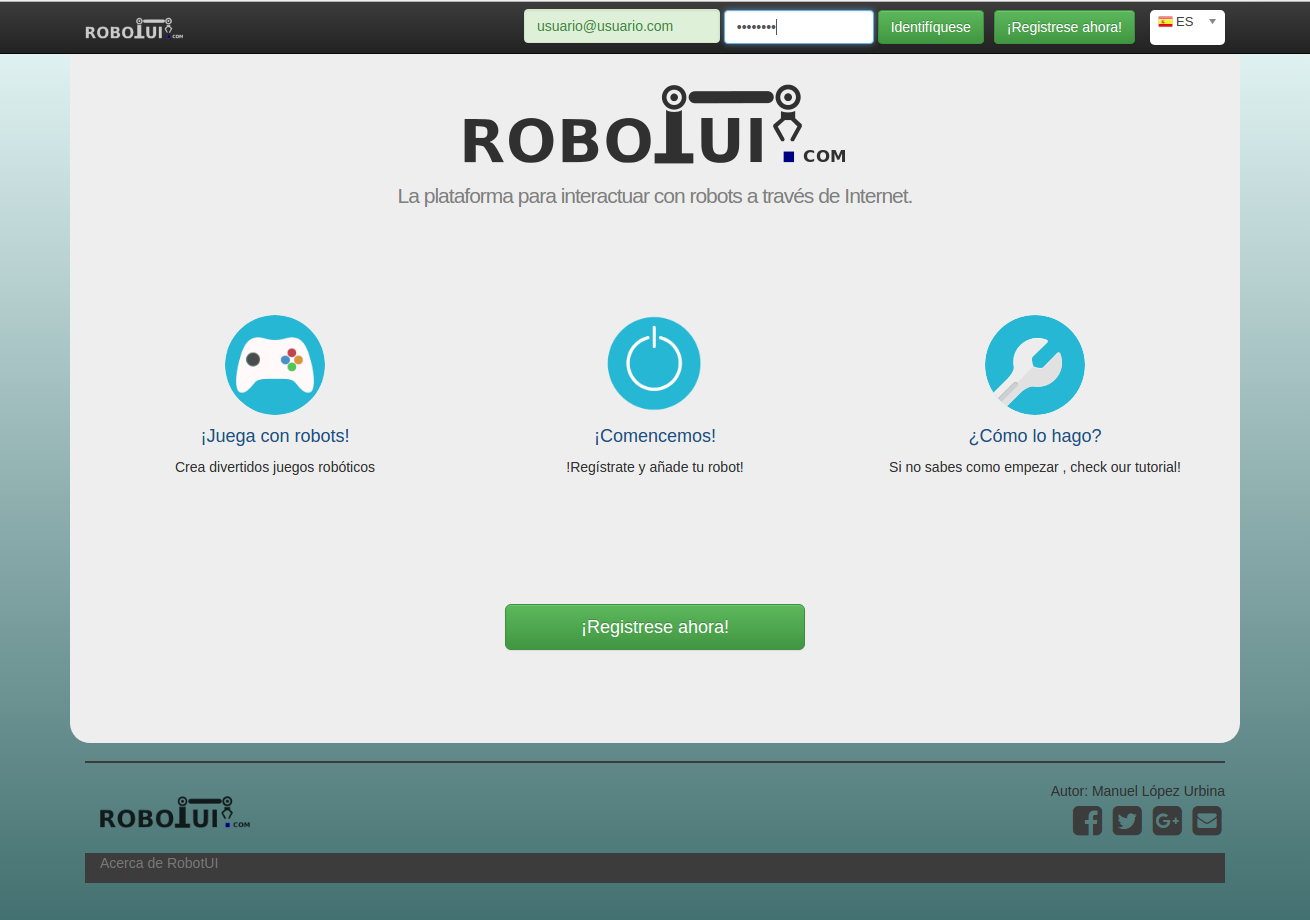
\includegraphics[scale=0.3]{imagenes/manual-usuario/pagina-principal.png}
  \end{center}
  \label{fig:logo}
 \caption{Página principal de RobotUI.}
\end{figure}


El elemento hardware de este proyecto se compone de un vehículo controlado vía WiFi el cual responde a una serie de señales, \emph{comandos}\footnote{ Comando: instrucción u orden que el usuario proporciona a un sistema informático, 
desde la línea de comandos (como una shell) o desde una llamada de programación.}, a los que responde realizando determinadas acciones. Por otra parte también dispone de una cámara para la captura de imágenes.\\

La interfaz de control generada en la aplicación web se configurará de tal manera que permita el control del susodicho vehículo a modo demostrativo. Este procedimiento servirá de guía para que cualquier usuario pueda proceder a dar de alta sus dispositivos 
robóticos para su control y difusión con otros usuarios.\\

\begin{figure}[H]
  \begin{center}
    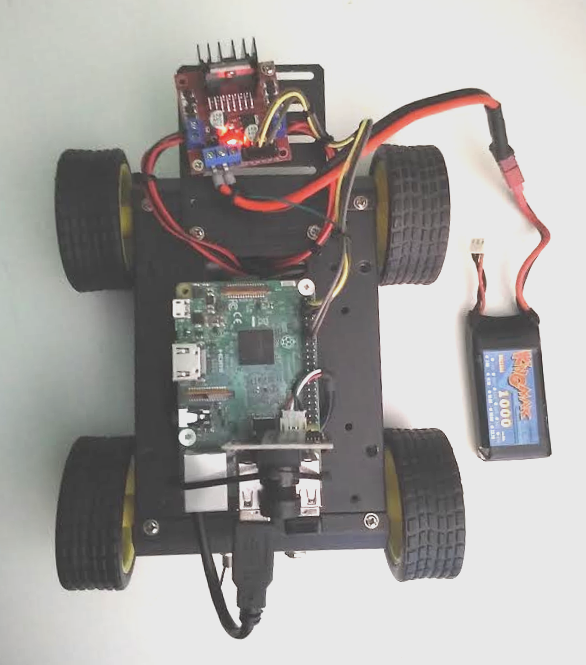
\includegraphics[scale=0.3]{imagenes/robot.jpg}
  \end{center}
  \label{fig:logo}
 \caption{Imagen del vehículo de pruebas desarrollado \protect\footnotemark.}
\end{figure}

\footnotetext{Vehículo desarrollado para probar el funcionamiento de RobotUI. Su desarrollo y características quedan descritas en el capítulo \ref{chap:robot}.}


\section{Objetivos}
\label{sec:objetivos}

Como hemos visto, se requiere de multitud de conocimientos a la hora de afrontar un proyecto robótico con ciertas garantías. Este proyecto trata, al menos, de reducir, o facilitar, el área relacionada con
la informática, más concretamente con la programación donde multitud de personas ven un impedimento a la hora de comenzar a desarrollar sus ideas.\\

Por otro lado, existe la imperiosa necesidad de que los usuarios quieran mostrar sus creaciones al resto del mundo, compartir experiencias, problemas, opiniones, etc, de una forma directa y no
mediante la grabación de vídeos del funcionamiento de los proyectos robóticos en cuestión en la que solo se visualiza su funcionamiento sin la posibilidad de interactuar, ya que no disponen de una herramienta adecuada para ello.\\

De lo anterior deducimos que existe la necesidad de que otros usuarios puedan participar de manera más activa, ya sea visualizando el control del robot por parte de su creador o permitir que otros usuarios
tomen el control de esos proyectos en tiempo real.\\

El sistema a desarrollar dispondrá de dos modos de funcionamiento, el primero de ellos proporciona las herramientas para la configuración de una interfaz a gusto del usuario, en la cual, 
una vez configurada, el usuario podrá controlar a su antojo el dispositivo. En el segundo modo de funcionamiento, la aplicación permitirá que otros usuarios puedan visitar la interfaz anteriormente 
configurada y actuar como espectadores en el control del robot por el usuario propietario del mismo. En definitiva, se proporcionará un sistema de control y difusión en uno solo.\\


En resumen, este proyecto busca facilitar la árdua labor de programación de los proyectos robóticos junto con la posibilidad de compartir las creaciones realizadas con otros usuarios.\\


\section{Acerca de este documento}

El documento se ha sido elaborado en un lenguaje claro y sencillo para permitir que un estudiante universitario de Ingeniería Informática pueda comprender los contenidos sin apenas dificultad añadida.\\

Este documento se organiza en los siguientes capítulos:\\

\begin{itemize}

\item En el capítulo \ref{chap:introducción}, Introducción, se comentan las razones que han motivado la creación de este proyecto, así como el propósito del mismo.

\item En el capítulo \ref{chap:conceptos-básicos}, Conceptos básicos, se incluyen definiciones de aquellos conceptos considerados de interés para la correcta comprensión del contenido de la presente memoria.

\item En el capítulo \ref{chap:herramientas}, Estado del arte y herramientas utilizadas, se realiza una descripción de las diferentes elementos hardware y software empleados durante el desarrollo del proyecto y necesarios para la utilización del mismo. Así como una breve descripción del conocimiento acumulado y tecnologías existentes hasta la fecha.

\item En el capítulo \ref{chap:desarrollo-software}, Desarrollo software, se realiza un análisis sobre la metodología empleada para el desarrollo software, describiendo los modelos de ciclo de vida utilizados, la descripción de los requisitos funcionales y no funcionales junto con los diagramas de casos de uso, de clases y de secuencia.

\item En el capítulo \ref{chap:desarrollo-frontend}, Desarrollo front-end, se recogen aquellos aspectos técnicos de interés referentes a la elaboración de toda la parte visual de la aplicación.

\item En el capítulo \ref{chap:comunicaciones}, Comunicaciones, se hace una descripción de las diferentes herramientas proporcionadas por el SDK del framework Sails.js para la gestión de eventos en tiempo real y la descripción de su funcionamiento mediante la explicación de casos prácticos desarrollados en el presente proyecto.

\item En el capítulo \ref{chap:robot}, Robot de pruebas, se recogen aquellos aspectos referentes al montaje, configuración y programación de un robot de pruebas para la demostración y uso de la aplicación desarrollada en el presente proyecto. 

\item En el capítulo \ref{chap:planificación}, Organización temporal, se recoge todo lo que concierne a la distribución y duración de cada una de las tareas llevadas a cabo durante el desarrollo del proyecto que el presente documento describe.

\item En el capítulo \ref{chap:manual-usuario}, Guía de usuario, se describen los diferentes aspectos necesarios para la correcta utilización del conjunto software y hardware de los que se compone el presente proyecto.

\item En el capítulo \ref{chap:conclusiones}, Comentarios finales, se hace mención de las conclusiones obtenidas tras la realización del proyecto además de las posibles mejoras aplicables y presupuesto.

\item En el apéndice Anexos \ref{appendix:anexos}, aparecen los manuales de instalación del software que ha sido necesario para la realización del proyecto.

\end{itemize}
